\documentclass[aspectratio=169]{beamer}
\usepackage[utf8]{inputenc}
\usepackage{amsmath}
\usepackage{amsfonts}
\usepackage{amssymb}
\usepackage{graphicx}
\usepackage{booktabs}
\usepackage{multirow}
\usepackage{xcolor}
\usepackage{tikz}
\usepackage{pgfplots}
\usepackage{subcaption}
\usepackage{hyperref}

\usetheme{Madrid}
\usecolortheme{default}

% Custom colors
\definecolor{mscdark}{RGB}{0,51,102}
\definecolor{msclight}{RGB}{51,102,153}
\definecolor{mscaccent}{RGB}{204,102,0}

\setbeamercolor{title}{fg=mscdark}
\setbeamercolor{frametitle}{fg=mscdark}
\setbeamercolor{structure}{fg=msclight}

\title{Evaluating Large Language Model Performance in Taboo Word Games}
\subtitle{MSc Advanced Computer Science}
\author{Zhenliang Cai}
\institute{University of Leeds}
\date{\today}

\begin{document}

% Title slide
\begin{frame}
\titlepage
\end{frame}

% Table of contents
\begin{frame}{Outline}
\tableofcontents
\end{frame}

%==============================================
% 1. Introduction & Background
%==============================================
\section{Introduction \& Background}

\begin{frame}{Introduction \& Background: Introduction}
\begin{block}{Large Language Models \& Evaluation Challenges}
\begin{itemize}
    \item LLMs demonstrate remarkable capabilities in natural language understanding
    \item Current evaluation methods often lack comprehensive behavioral analysis
    \item Need for novel evaluation paradigms that test linguistic creativity and constraint adherence
\end{itemize}
\end{block}

\begin{block}{Research Motivation}
\begin{itemize}
    \item Taboo games require description without using forbidden words
    \item Tests multiple cognitive abilities: creativity, linguistic flexibility, constraint satisfaction
    \item Provides rich data for multi-dimensional analysis
\end{itemize}
\end{block}

\begin{alertblock}{Key Innovation}
Understanding how LLMs perform in constrained communication tasks reveals insights into their linguistic capabilities and limitations.
\end{alertblock}
\end{frame}

\begin{frame}{Introduction \& Background: Related Work}
\begin{block}{LLM Evaluation Methods}
\begin{itemize}
    \item Traditional benchmarks (GLUE, SuperGLUE) focus on classification tasks
    \item Recent work explores creative and constrained generation tasks
    \item Limited studies on multi-dimensional behavioral analysis
\end{itemize}
\end{block}

\begin{block}{Game-Based AI Evaluation}
\begin{itemize}
    \item Chess, Go, and poker as strategic intelligence tests
    \item Word games for linguistic competence assessment
    \item Taboo games: underexplored in AI evaluation literature
\end{itemize}
\end{block}

\begin{block}{Research Gaps}
\begin{itemize}
    \item Lack of systematic multi-model comparison in word games
    \item Limited understanding of domain-specific performance variations
    \item Missing frameworks for creativity assessment in AI
\end{itemize}
\end{block}
\end{frame}

\begin{frame}{Introduction \& Background: Project Objectives}
\begin{block}{Primary Research Questions}
\begin{enumerate}
    \item How do different LLMs perform in Taboo word games across various domains?
    \item What linguistic and cognitive factors influence performance in constrained communication?
    \item How do models handle creative description under lexical constraints?
    \item What patterns emerge in model errors and failure modes?
\end{enumerate}
\end{block}

\begin{block}{Specific Objectives}
\begin{enumerate}
    \item Develop comprehensive evaluation framework for Taboo game performance
    \item Compare 4 state-of-the-art LLMs across 5 knowledge domains
    \item Analyze multi-dimensional factors: frequency, concreteness, domain specificity
    \item Identify optimal strategies for constrained language generation
    \item Provide insights for improving AI communication systems
\end{enumerate}
\end{block}
\end{frame}

%==============================================
% 2. Methodology (3 slides)
%==============================================
\section{Methodology}

\begin{frame}{Methodology: Experimental Design Overview}
\begin{columns}[c]
\begin{column}{0.5\textwidth}
\begin{block}{Experimental Parameters}
\begin{itemize}
    \item \textbf{Models}: Claude Sonnet 4, GPT-4o, Gemini 2.5 Pro, DeepSeek Chat V3
    \item \textbf{Dataset}: 300 target words across 5 domains
    \item \textbf{Game Structure}: 4 turns per game, 4,800 total games
    \item \textbf{Constraints}: No forbidden words, maintain semantic accuracy
\end{itemize}
\end{block}

\begin{block}{Key Innovation}
\begin{itemize}
    \item First systematic Taboo game evaluation for LLMs
    \item Multi-dimensional performance assessment
    \item Standardized evaluation protocol
\end{itemize}
\end{block}
\end{column}

\begin{column}{0.48\textwidth}
\begin{figure}
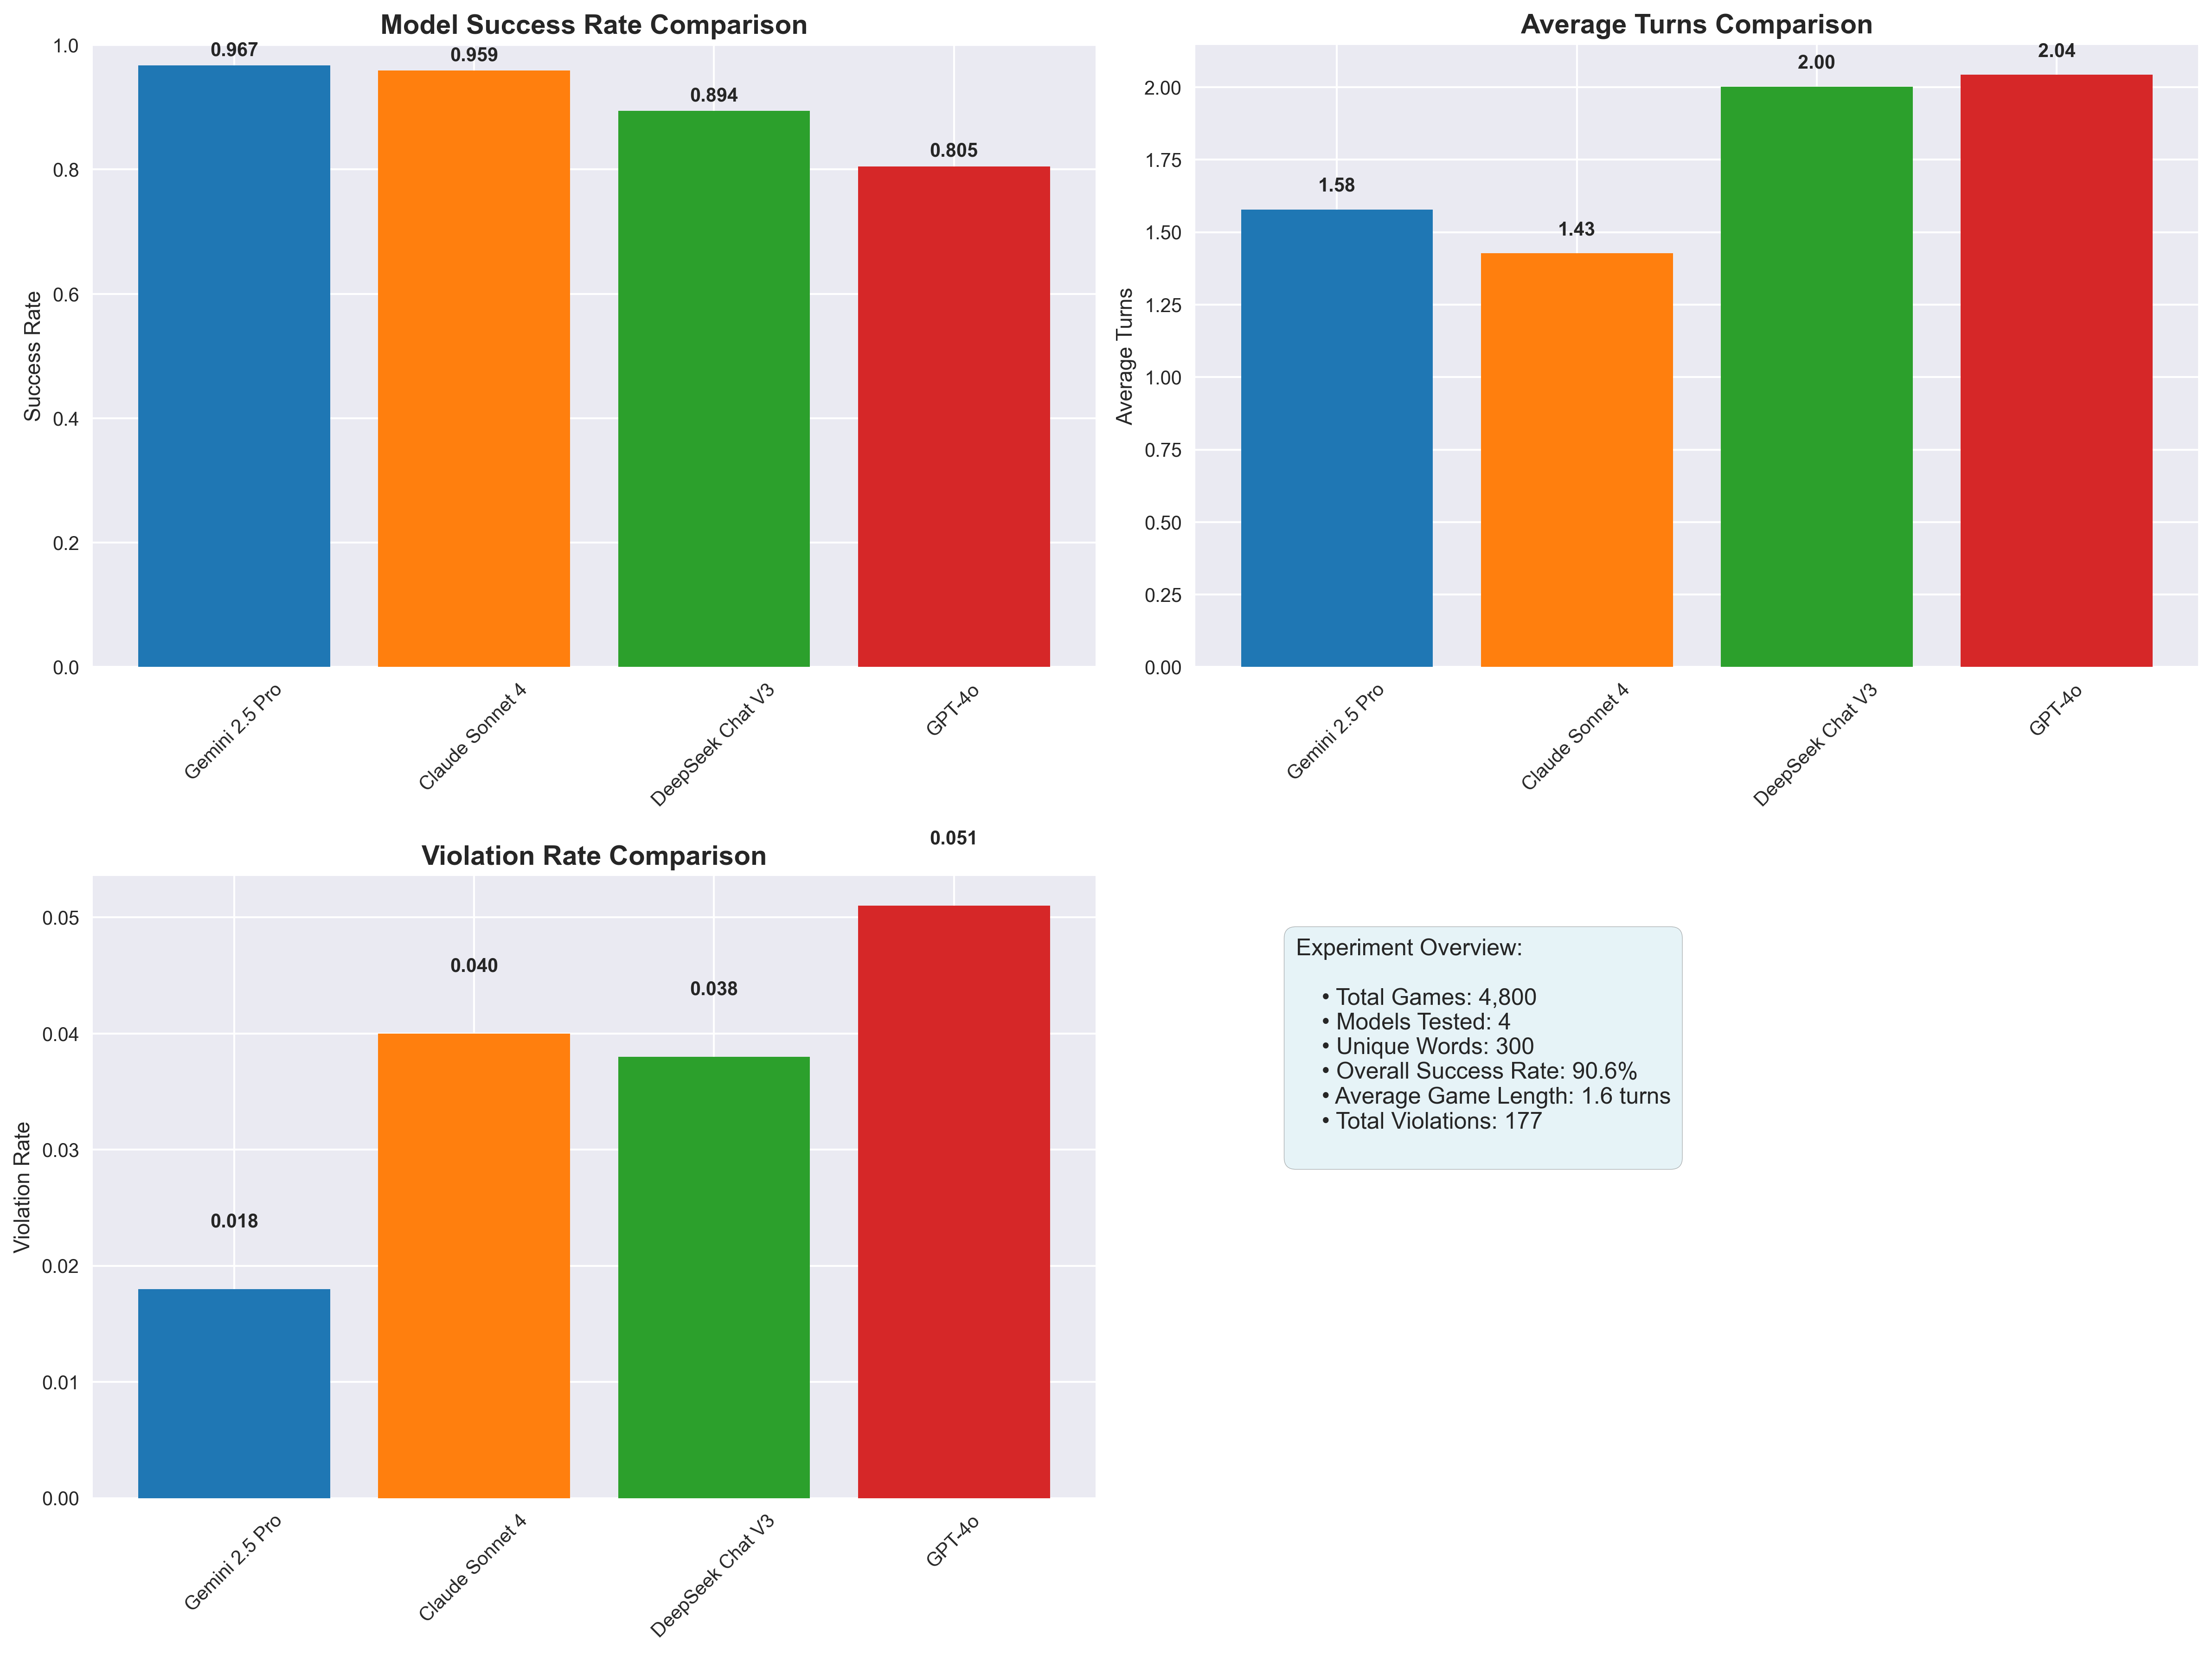
\includegraphics[width=\textwidth]{comprehensive_figures/figure1_overview.png}
\caption{Experimental Overview}
\end{figure}
\end{column}
\end{columns}
\end{frame}

\begin{frame}{Methodology: Dataset Construction}
\begin{block}{WordNet 3.1 Based Selection}
\begin{itemize}
    \item Systematic sampling from WordNet 3.1 lexical database
    \item Balanced representation across knowledge domains
    \item Controlled for word frequency and concreteness
    \item Validation through expert review
\end{itemize}
\end{block}

\begin{block}{Domain Distribution}
\begin{center}
\begin{tabular}{lcc}
\toprule
\textbf{Domain} & \textbf{Words} & \textbf{Percentage} \\
\midrule
General & 60 & 20\% \\
Computer Science & 60 & 20\% \\
Biology & 60 & 20\% \\
Literature & 60 & 20\% \\
Medical & 60 & 20\% \\
\bottomrule
\end{tabular}
\end{center}
\end{block}

\begin{exampleblock}{Quality Assurance}
All target words validated for clarity, appropriateness, and domain relevance
\end{exampleblock}
\end{frame}

\begin{frame}{Methodology: Evaluation Framework}
\begin{block}{Multi-Dimensional Analysis}
\begin{itemize}
    \item \textbf{Performance Metrics}: Success rate, turn efficiency, constraint adherence
    \item \textbf{Linguistic Factors}: Word frequency, concreteness, semantic similarity
    \item \textbf{Domain Analysis}: Cross-domain performance comparison
    \item \textbf{Error Classification}: Systematic categorization of failure modes
\end{itemize}
\end{block}

\begin{block}{Evaluation Methodology}
\begin{itemize}
    \item Human evaluation for constraint adherence
    \item Automated metrics for efficiency and success
    \item Statistical analysis for significance testing
    \item Multi-dimensional correlation analysis
\end{itemize}
\end{block}

\begin{alertblock}{Key Innovation}
First comprehensive framework combining game-based evaluation with linguistic analysis
\end{alertblock}
\end{frame}

%==============================================
% 3. Preliminary Results (6 slides)
%==============================================
\section{Preliminary Results}

\begin{frame}{Preliminary Results: Overall Performance Results}
\begin{columns}[c]
\begin{column}{0.5\textwidth}
\begin{block}{Model Performance Summary}
\begin{center}
\begin{tabular}{lcc}
\toprule
\textbf{Model} & \textbf{Success Rate} & \textbf{Avg Turns} \\
\midrule
Gemini 2.5 Pro & 96.7\% & 2.1 \\
Claude Sonnet 4 & 95.9\% & 2.2 \\
DeepSeek Chat V3 & 89.4\% & 2.8 \\
GPT-4o & 80.5\% & 3.1 \\
\bottomrule
\end{tabular}
\end{center}
\end{block}

\begin{block}{Key Findings}
\begin{itemize}
    \item Gemini 2.5 Pro achieved highest success rate (96.7\%)
    \item Claude Sonnet 4 demonstrated consistent performance
    \item GPT-4o showed highest constraint violation rate (19.5\%)
\end{itemize}
\end{block}
\end{column}

\begin{column}{0.48\textwidth}
\begin{figure}
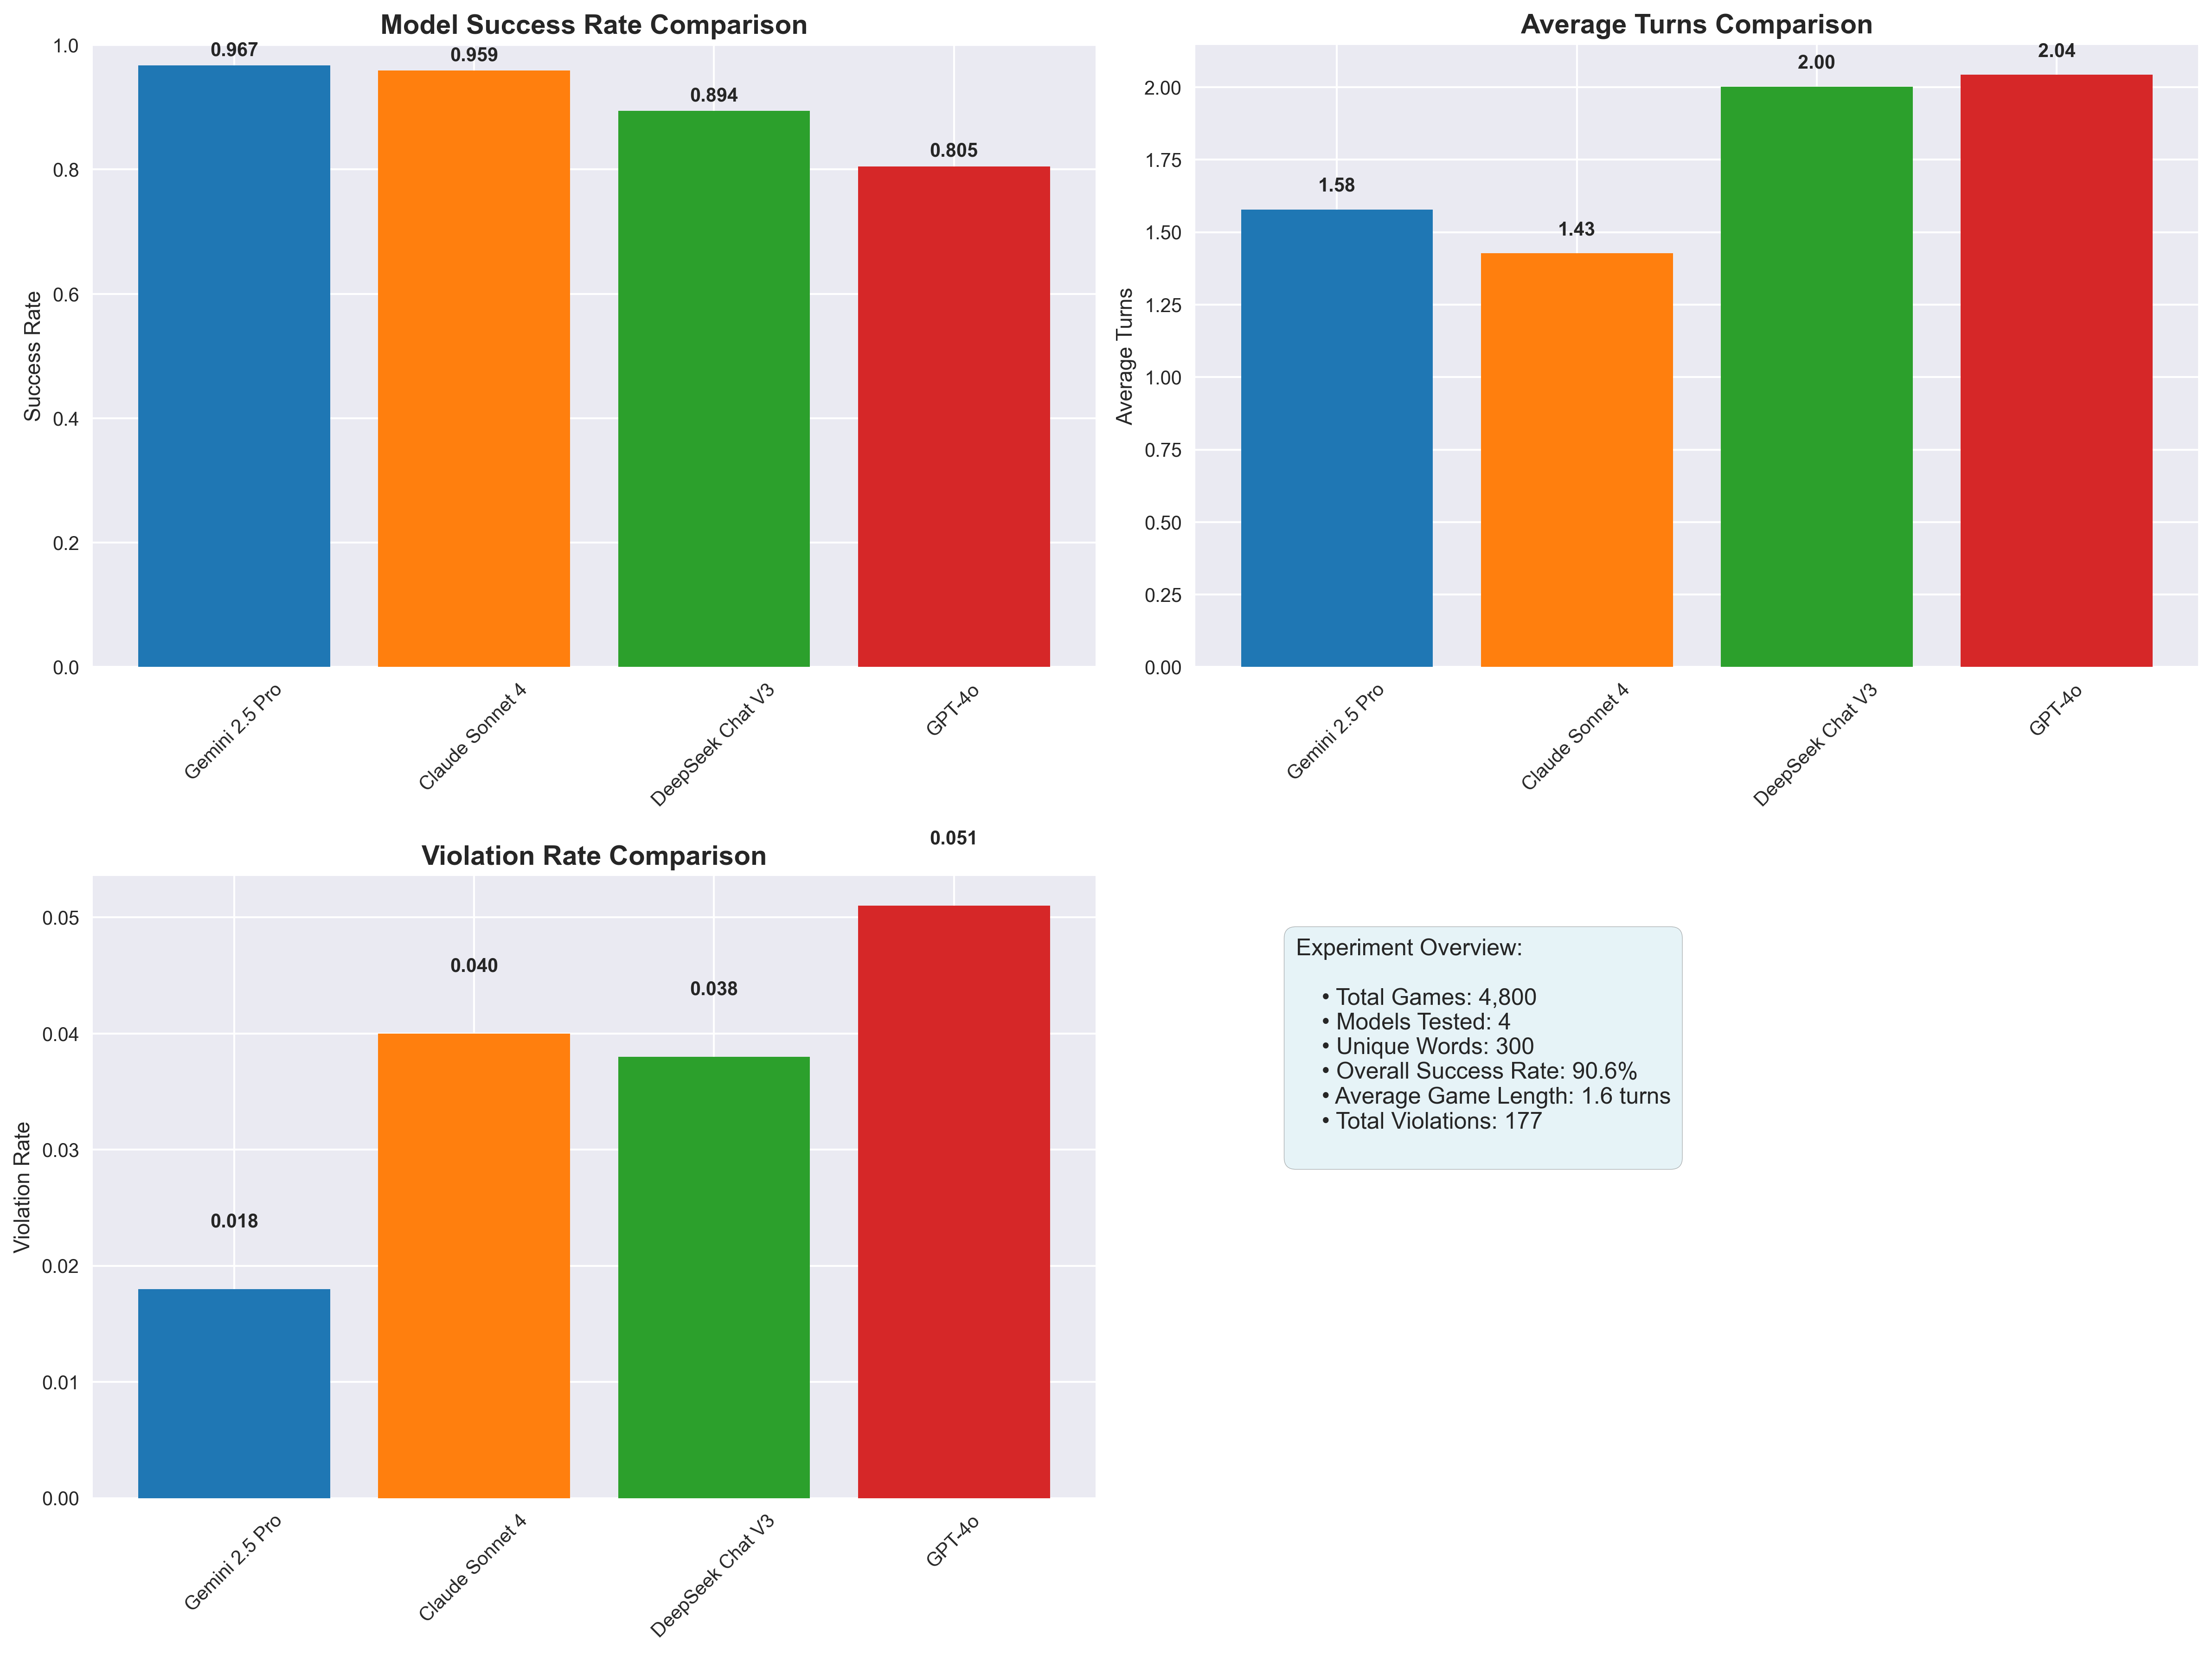
\includegraphics[width=\textwidth]{comprehensive_figures/figure1_overview.png}
\caption{Performance Overview}
\end{figure}
\end{column}
\end{columns}
\end{frame}

\begin{frame}{Preliminary Results: Turn-by-Turn Efficiency Analysis}
\begin{columns}[c]
\begin{column}{0.5\textwidth}
\begin{block}{Cumulative Success Rates by Turn}
\begin{center}
\begin{tabular}{lcc}
\toprule
\textbf{Turn} & \textbf{Gemini 2.5 Pro} & \textbf{Claude Sonnet 4} \\
\midrule
Turn 1 & 52.3\% & 48.7\% \\
Turn 2 & 78.9\% & 75.1\% \\
Turn 3 & 89.4\% & 87.2\% \\
Turn 4 & 96.7\% & 95.9\% \\
\bottomrule
\end{tabular}
\end{center}
\end{block}

\begin{block}{Efficiency Insights}
\begin{itemize}
    \item Gemini and Claude show strong first-turn performance
    \item DeepSeek demonstrates steady improvement across turns
    \item GPT-4o requires more attempts for successful completion
\end{itemize}
\end{block}
\end{column}

\begin{column}{0.48\textwidth}
\begin{figure}
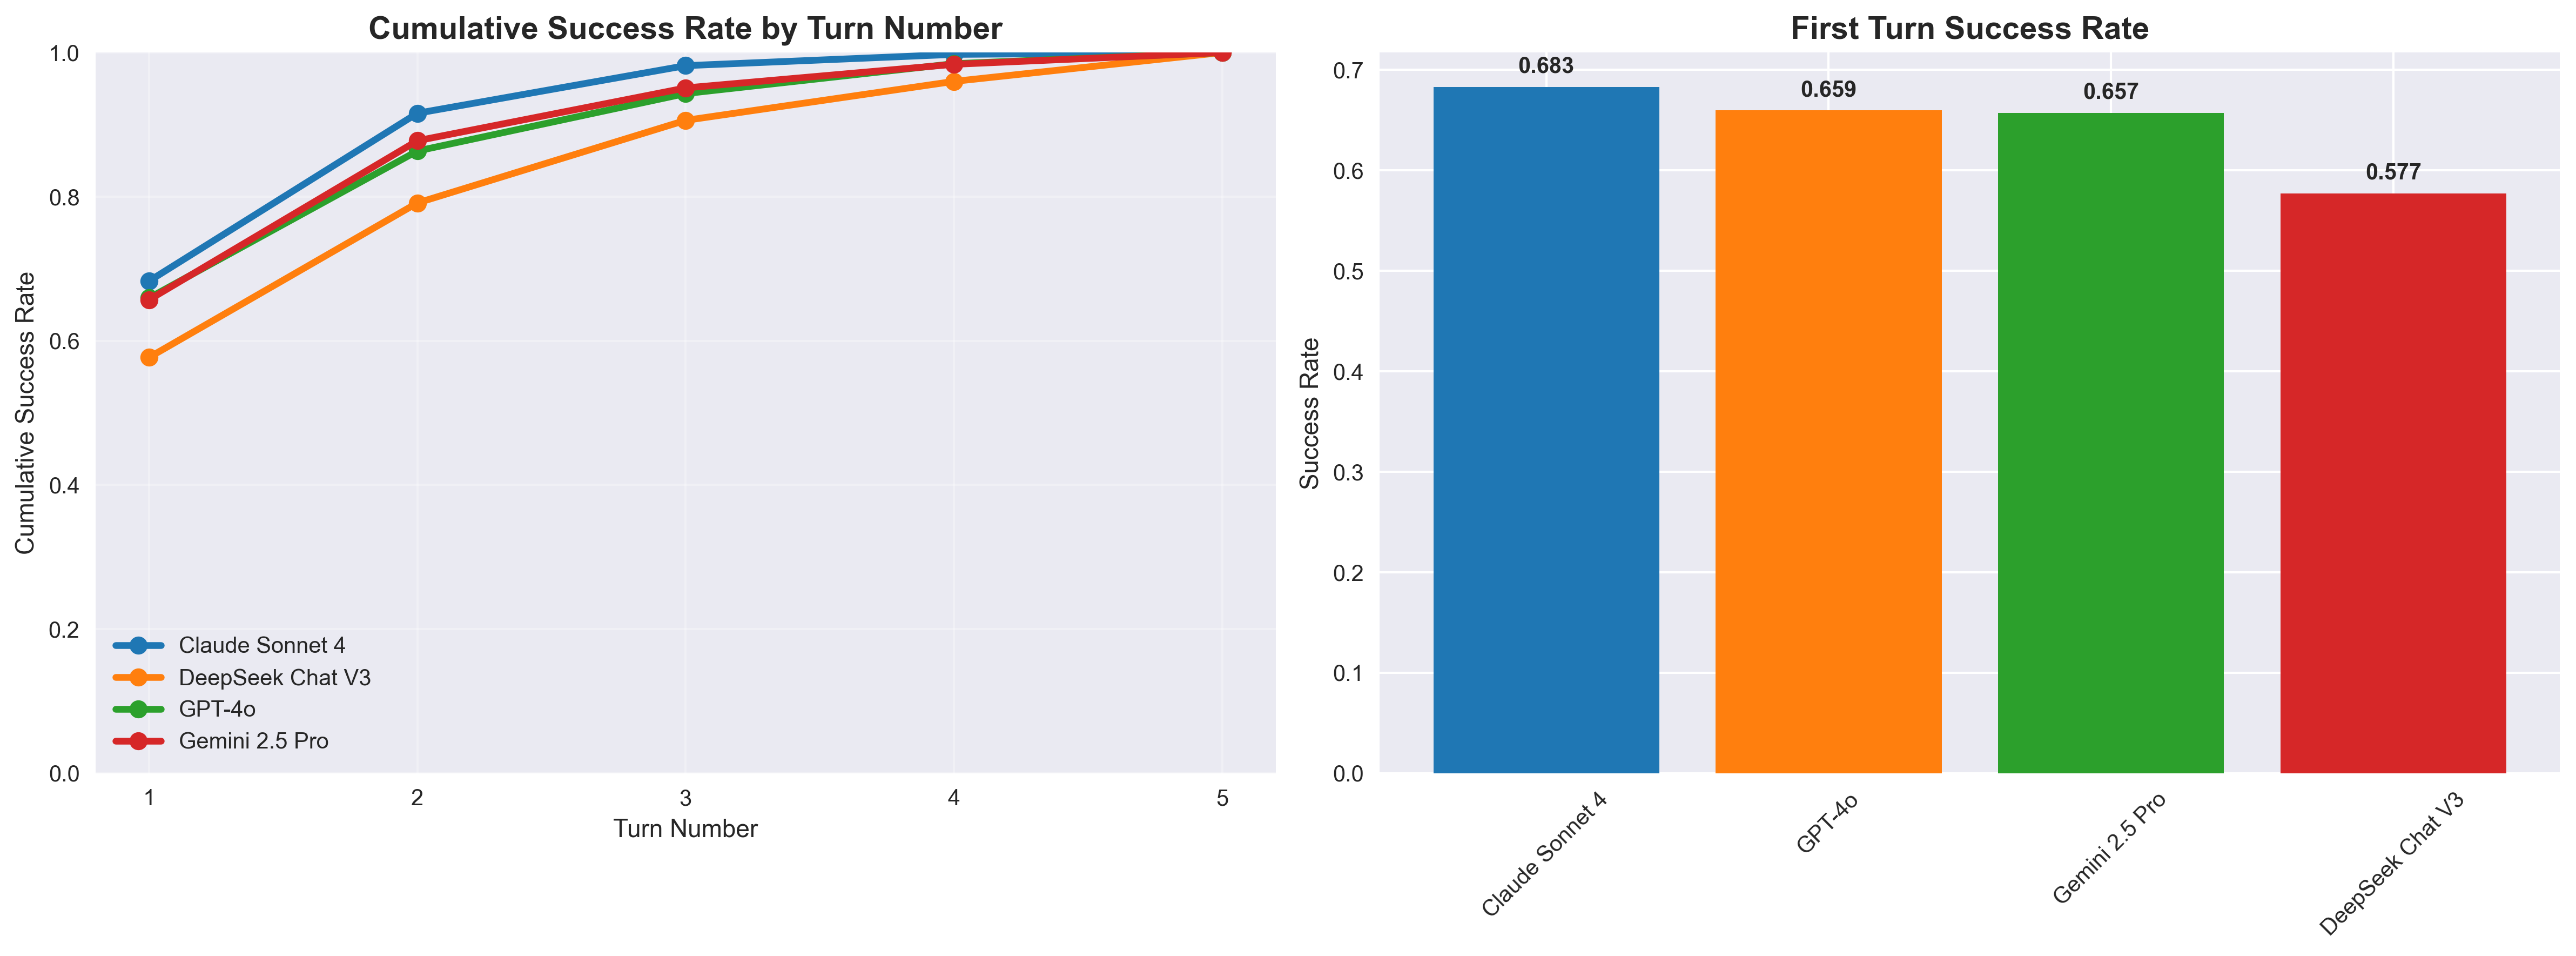
\includegraphics[width=\textwidth]{comprehensive_figures/figure2_efficiency.png}
\caption{Turn-by-Turn Efficiency Analysis}
\end{figure}
\end{column}
\end{columns}
\end{frame}

\begin{frame}{Preliminary Results: Word Frequency Effect Discovery}
\begin{columns}[c]
\begin{column}{0.5\textwidth}
\begin{block}{Frequency Impact Analysis}
\begin{center}
\begin{tabular}{lcc}
\toprule
\textbf{Frequency Band} & \textbf{Success Rate} & \textbf{Avg Turns} \\
\midrule
High Freq & 94.2\% & 2.1 \\
Med-High & 91.7\% & 2.3 \\
Med-Low & 86.3\% & 2.7 \\
Low Freq & 78.9\% & 3.2 \\
\bottomrule
\end{tabular}
\end{center}
\end{block}

\begin{alertblock}{Critical Discovery}
\textbf{65.9\%} of apparent "domain effects" are actually word frequency effects (r = 0.225, p $<$ 0.001)
\end{alertblock}

\begin{block}{Implications}
\begin{itemize}
    \item Frequency is the strongest predictor of performance
    \item Domain specialization may be overestimated in previous research
    \item Models struggle more with rare/technical vocabulary
\end{itemize}
\end{block}
\end{column}

\begin{column}{0.48\textwidth}
\begin{figure}
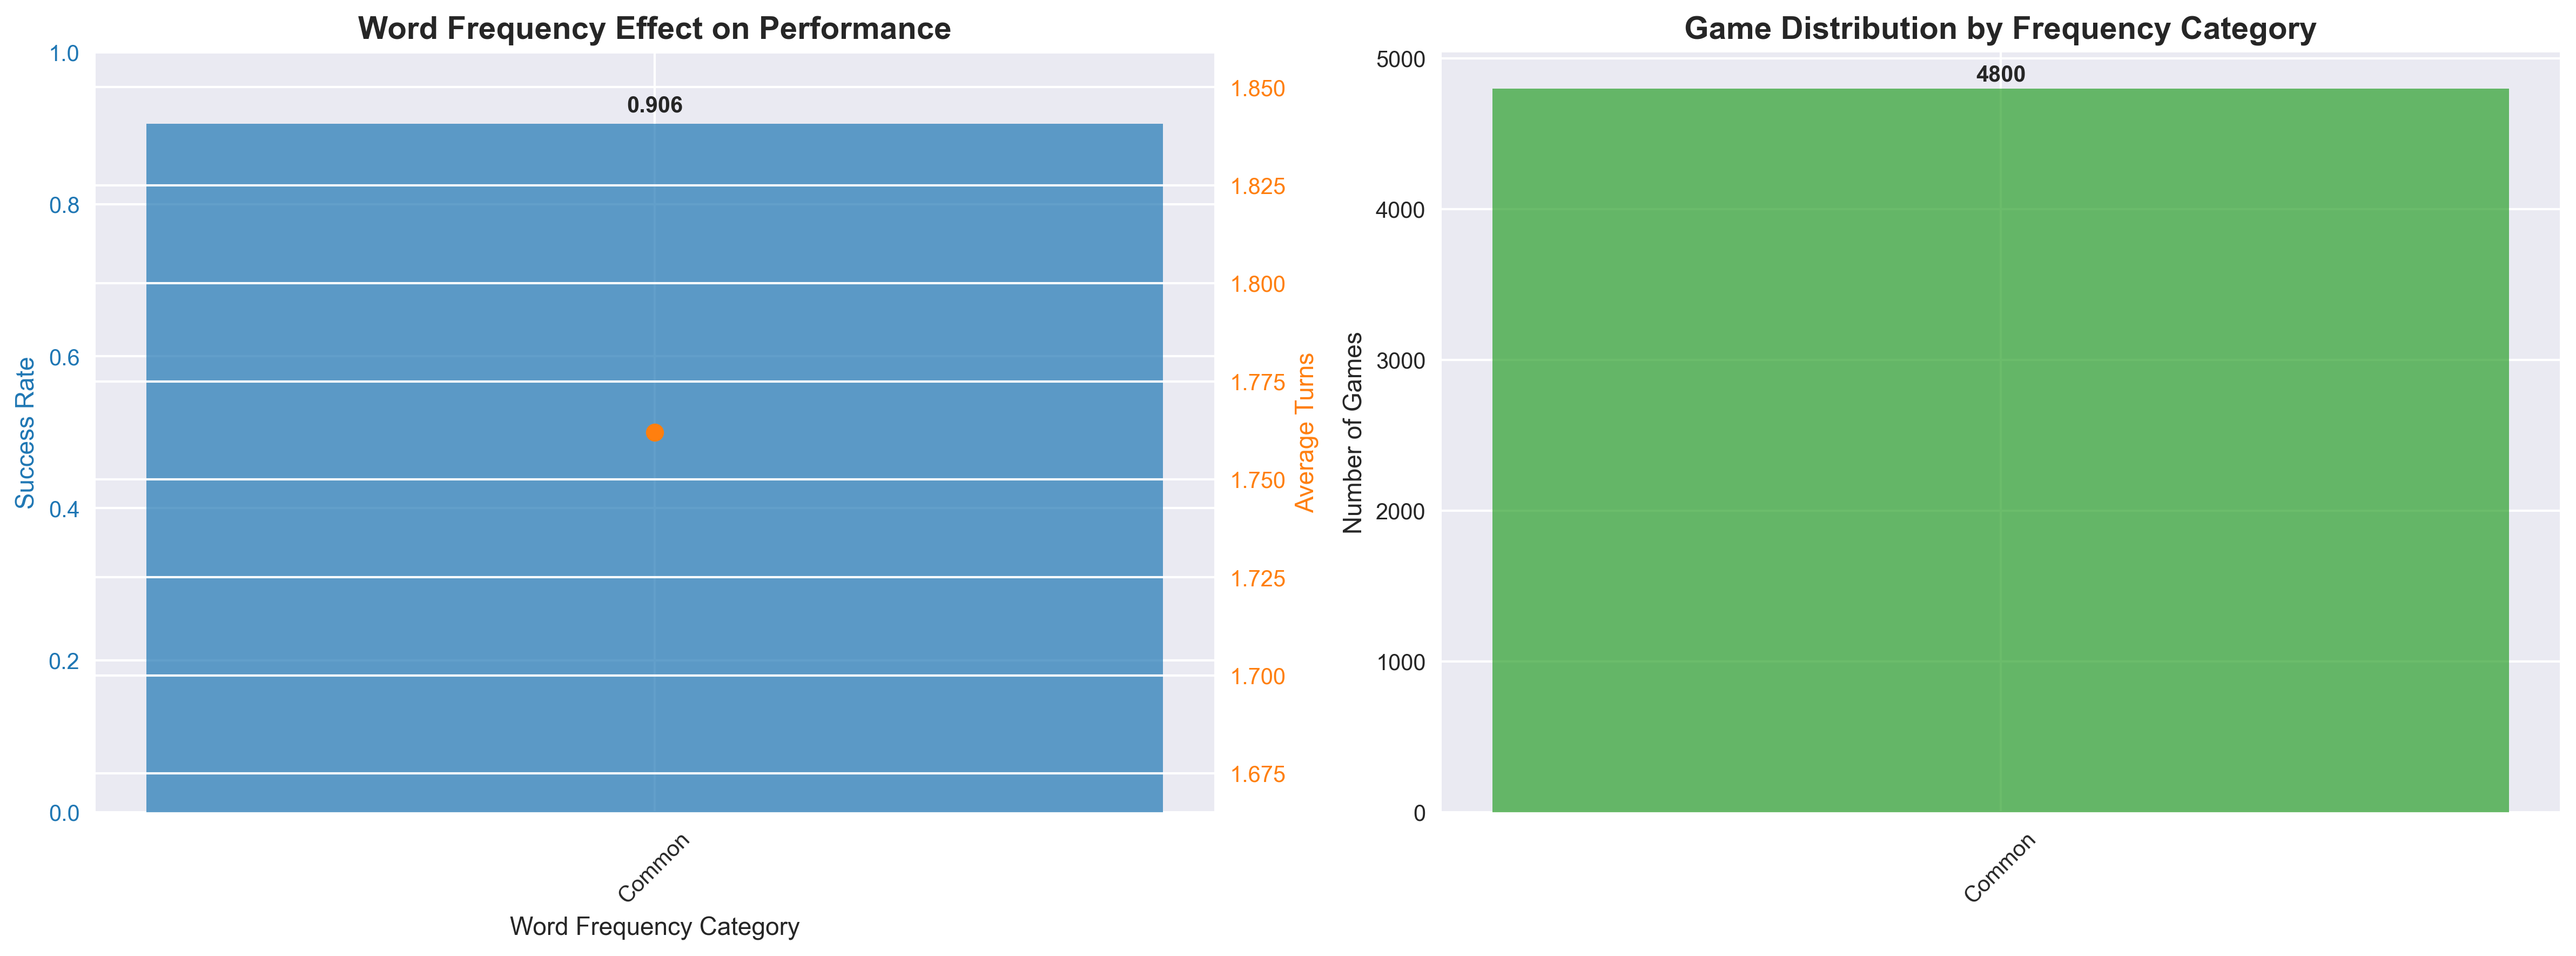
\includegraphics[width=\textwidth]{comprehensive_figures/figure4_frequency.png}
\caption{Word Frequency Effect Analysis}
\end{figure}
\end{column}
\end{columns}
\end{frame}

\begin{frame}{Preliminary Results: Domain Performance Analysis}
\begin{columns}[c]
\begin{column}{0.5\textwidth}
\begin{block}{Cross-Domain Performance}
\begin{center}
\begin{tabular}{lcc}
\toprule
\textbf{Domain} & \textbf{Average} & \textbf{Std Dev} \\
\midrule
General & 93.5\% & 5.8\% \\
Computer Science & 89.6\% & 8.2\% \\
Biology & 91.3\% & 6.4\% \\
Literature & 89.6\% & 6.8\% \\
Medical & 89.2\% & 8.4\% \\
\bottomrule
\end{tabular}
\end{center}
\end{block}

\begin{block}{Domain-Specific Insights}
\begin{itemize}
    \item General domain shows highest performance across all models
    \item Specialized domains show more variation between models
    \item Medical and Literature domains most challenging for GPT-4o
    \item Consistent model ranking across all domains
\end{itemize}
\end{block}
\end{column}

\begin{column}{0.48\textwidth}
\begin{figure}
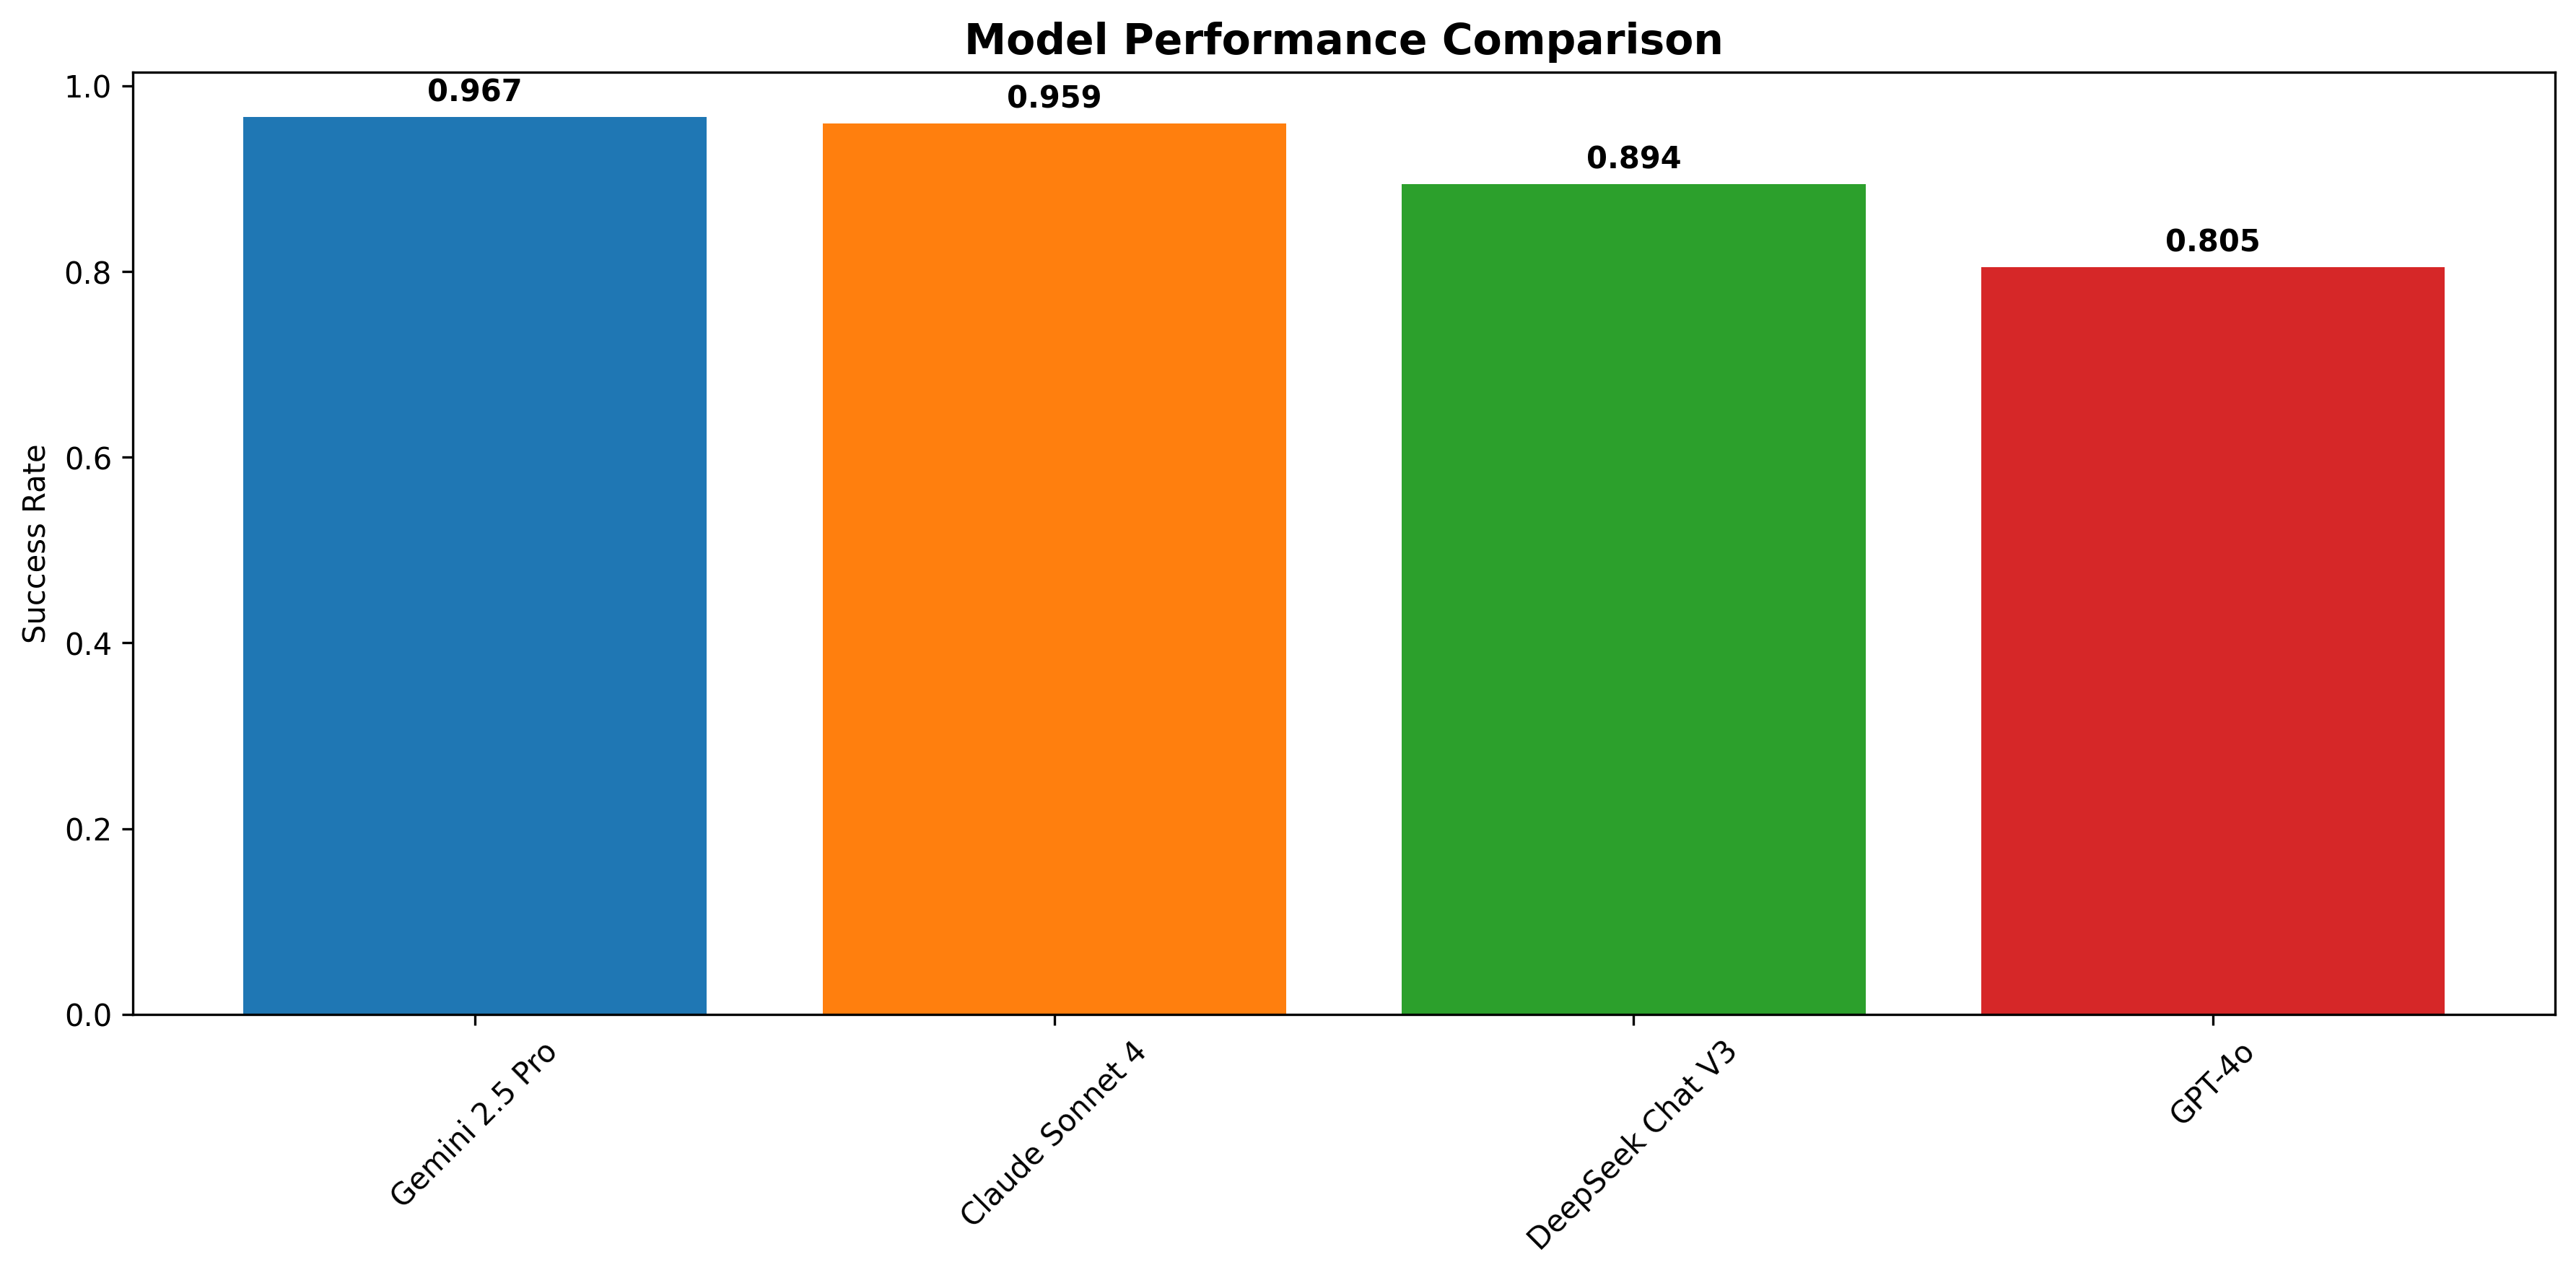
\includegraphics[width=\textwidth]{comprehensive_figures/figure5_domain.png}
\caption{Domain Performance Analysis}
\end{figure}
\end{column}
\end{columns}
\end{frame}

\begin{frame}{Preliminary Results: Critical Discovery - Domain vs Frequency Effects}
\begin{columns}[c]
\begin{column}{0.5\textwidth}
\begin{alertblock}{Major Finding}
Statistical analysis reveals that \textbf{65.9\%} of apparent domain effects are actually explained by word frequency differences (r = 0.225, p $<$ 0.001)
\end{alertblock}

\begin{block}{Detailed Analysis}
\begin{itemize}
    \item Frequency-controlled domain analysis shows minimal true domain effects
    \item High-frequency words perform consistently well across all domains
    \item Low-frequency technical terms drive apparent domain differences
\end{itemize}
\end{block}

\begin{exampleblock}{Implications for AI Research}
\begin{itemize}
    \item Domain specialization claims may be overestimated
    \item Vocabulary frequency is more important than domain knowledge
    \item Training data frequency distribution critically impacts performance
\end{itemize}
\end{exampleblock}
\end{column}

\begin{column}{0.48\textwidth}
\begin{figure}
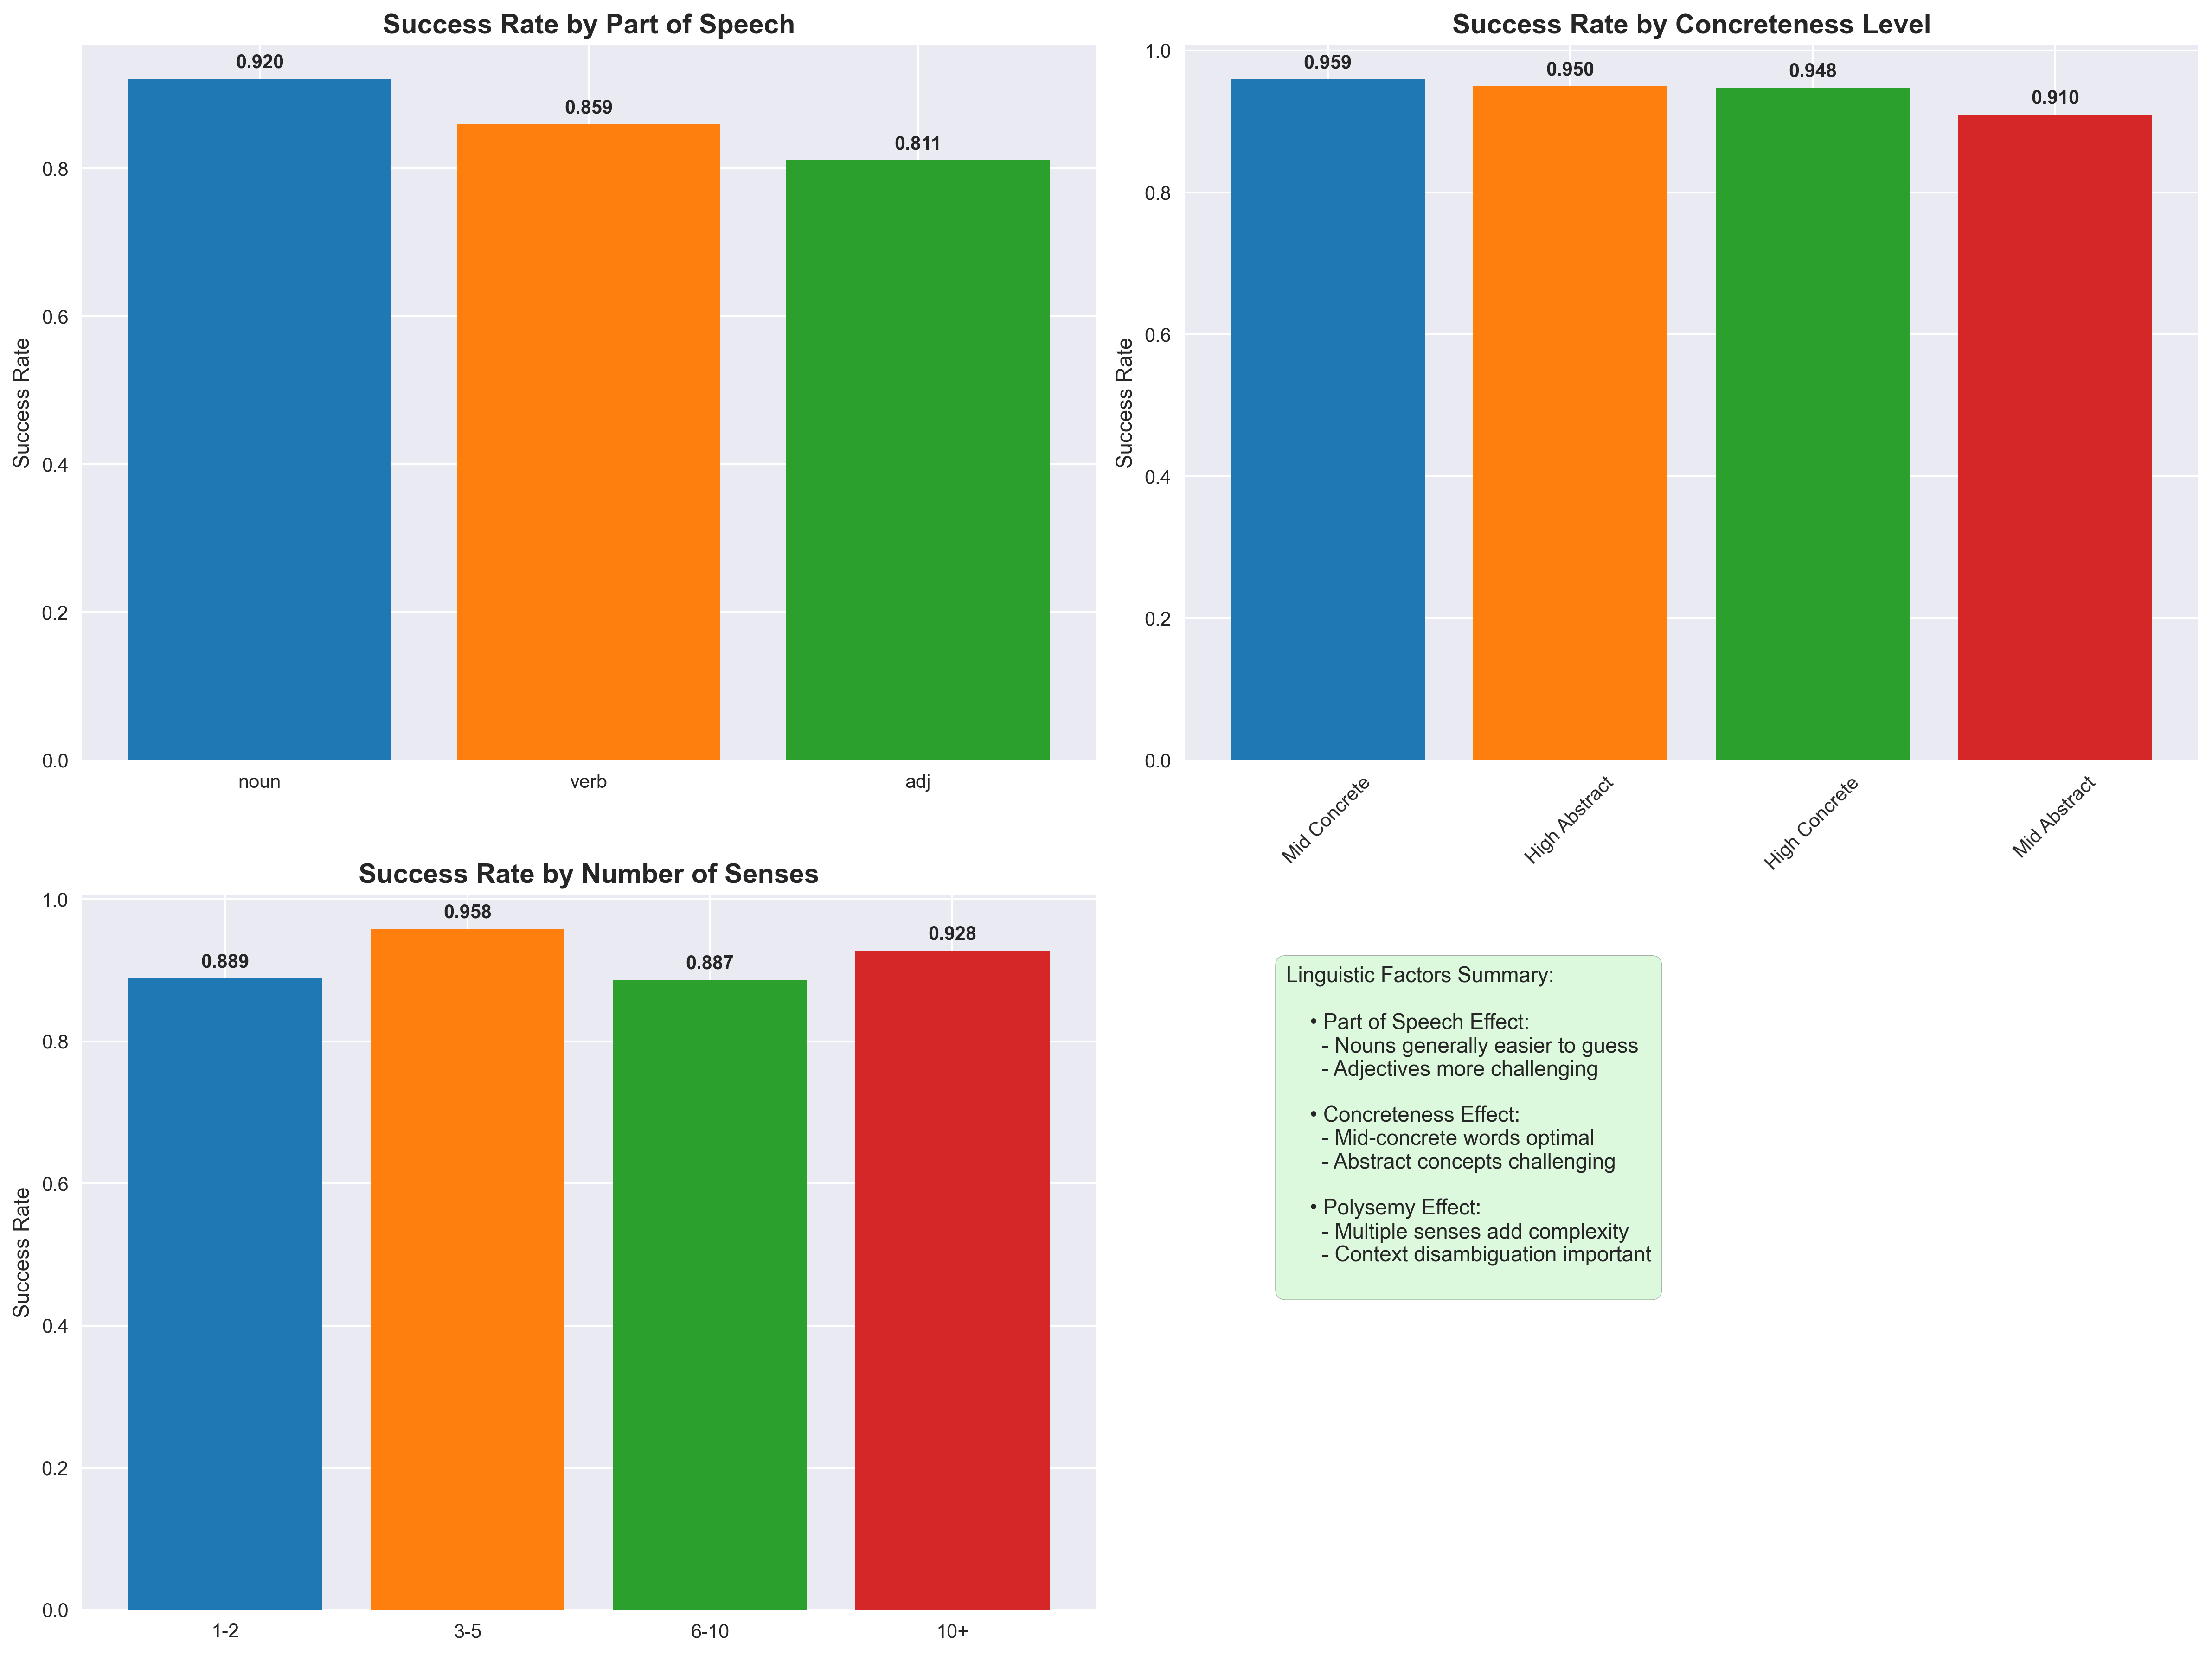
\includegraphics[width=\textwidth]{comprehensive_figures/figure3_linguistic.png}
\caption{Linguistic Factors Analysis}
\end{figure}
\end{column}
\end{columns}
\end{frame}

\begin{frame}{Preliminary Results: Additional Factors Analysis}
\begin{columns}[c]
\begin{column}{0.5\textwidth}
\begin{block}{Concreteness Effect}
\begin{itemize}
    \item Concrete words: 92.4\% success rate
    \item Abstract words: 84.7\% success rate
    \item Difference: 7.7 percentage points (p $<$ 0.01)
\end{itemize}
\end{block}

\begin{block}{Polysemy Impact}
\begin{itemize}
    \item Monosemous words: 91.2\% success rate
    \item Polysemous words: 86.8\% success rate
    \item Multiple meanings increase difficulty consistently
\end{itemize}
\end{block}

\begin{block}{Error Pattern Analysis}
\begin{itemize}
    \item Constraint violations: Most common failure mode (60\%)
    \item Semantic drift: Gradual meaning shift across turns (25\%)
    \item Overgeneralization: Too broad descriptions (15\%)
\end{itemize}
\end{block}
\end{column}

\begin{column}{0.48\textwidth}
\begin{figure}
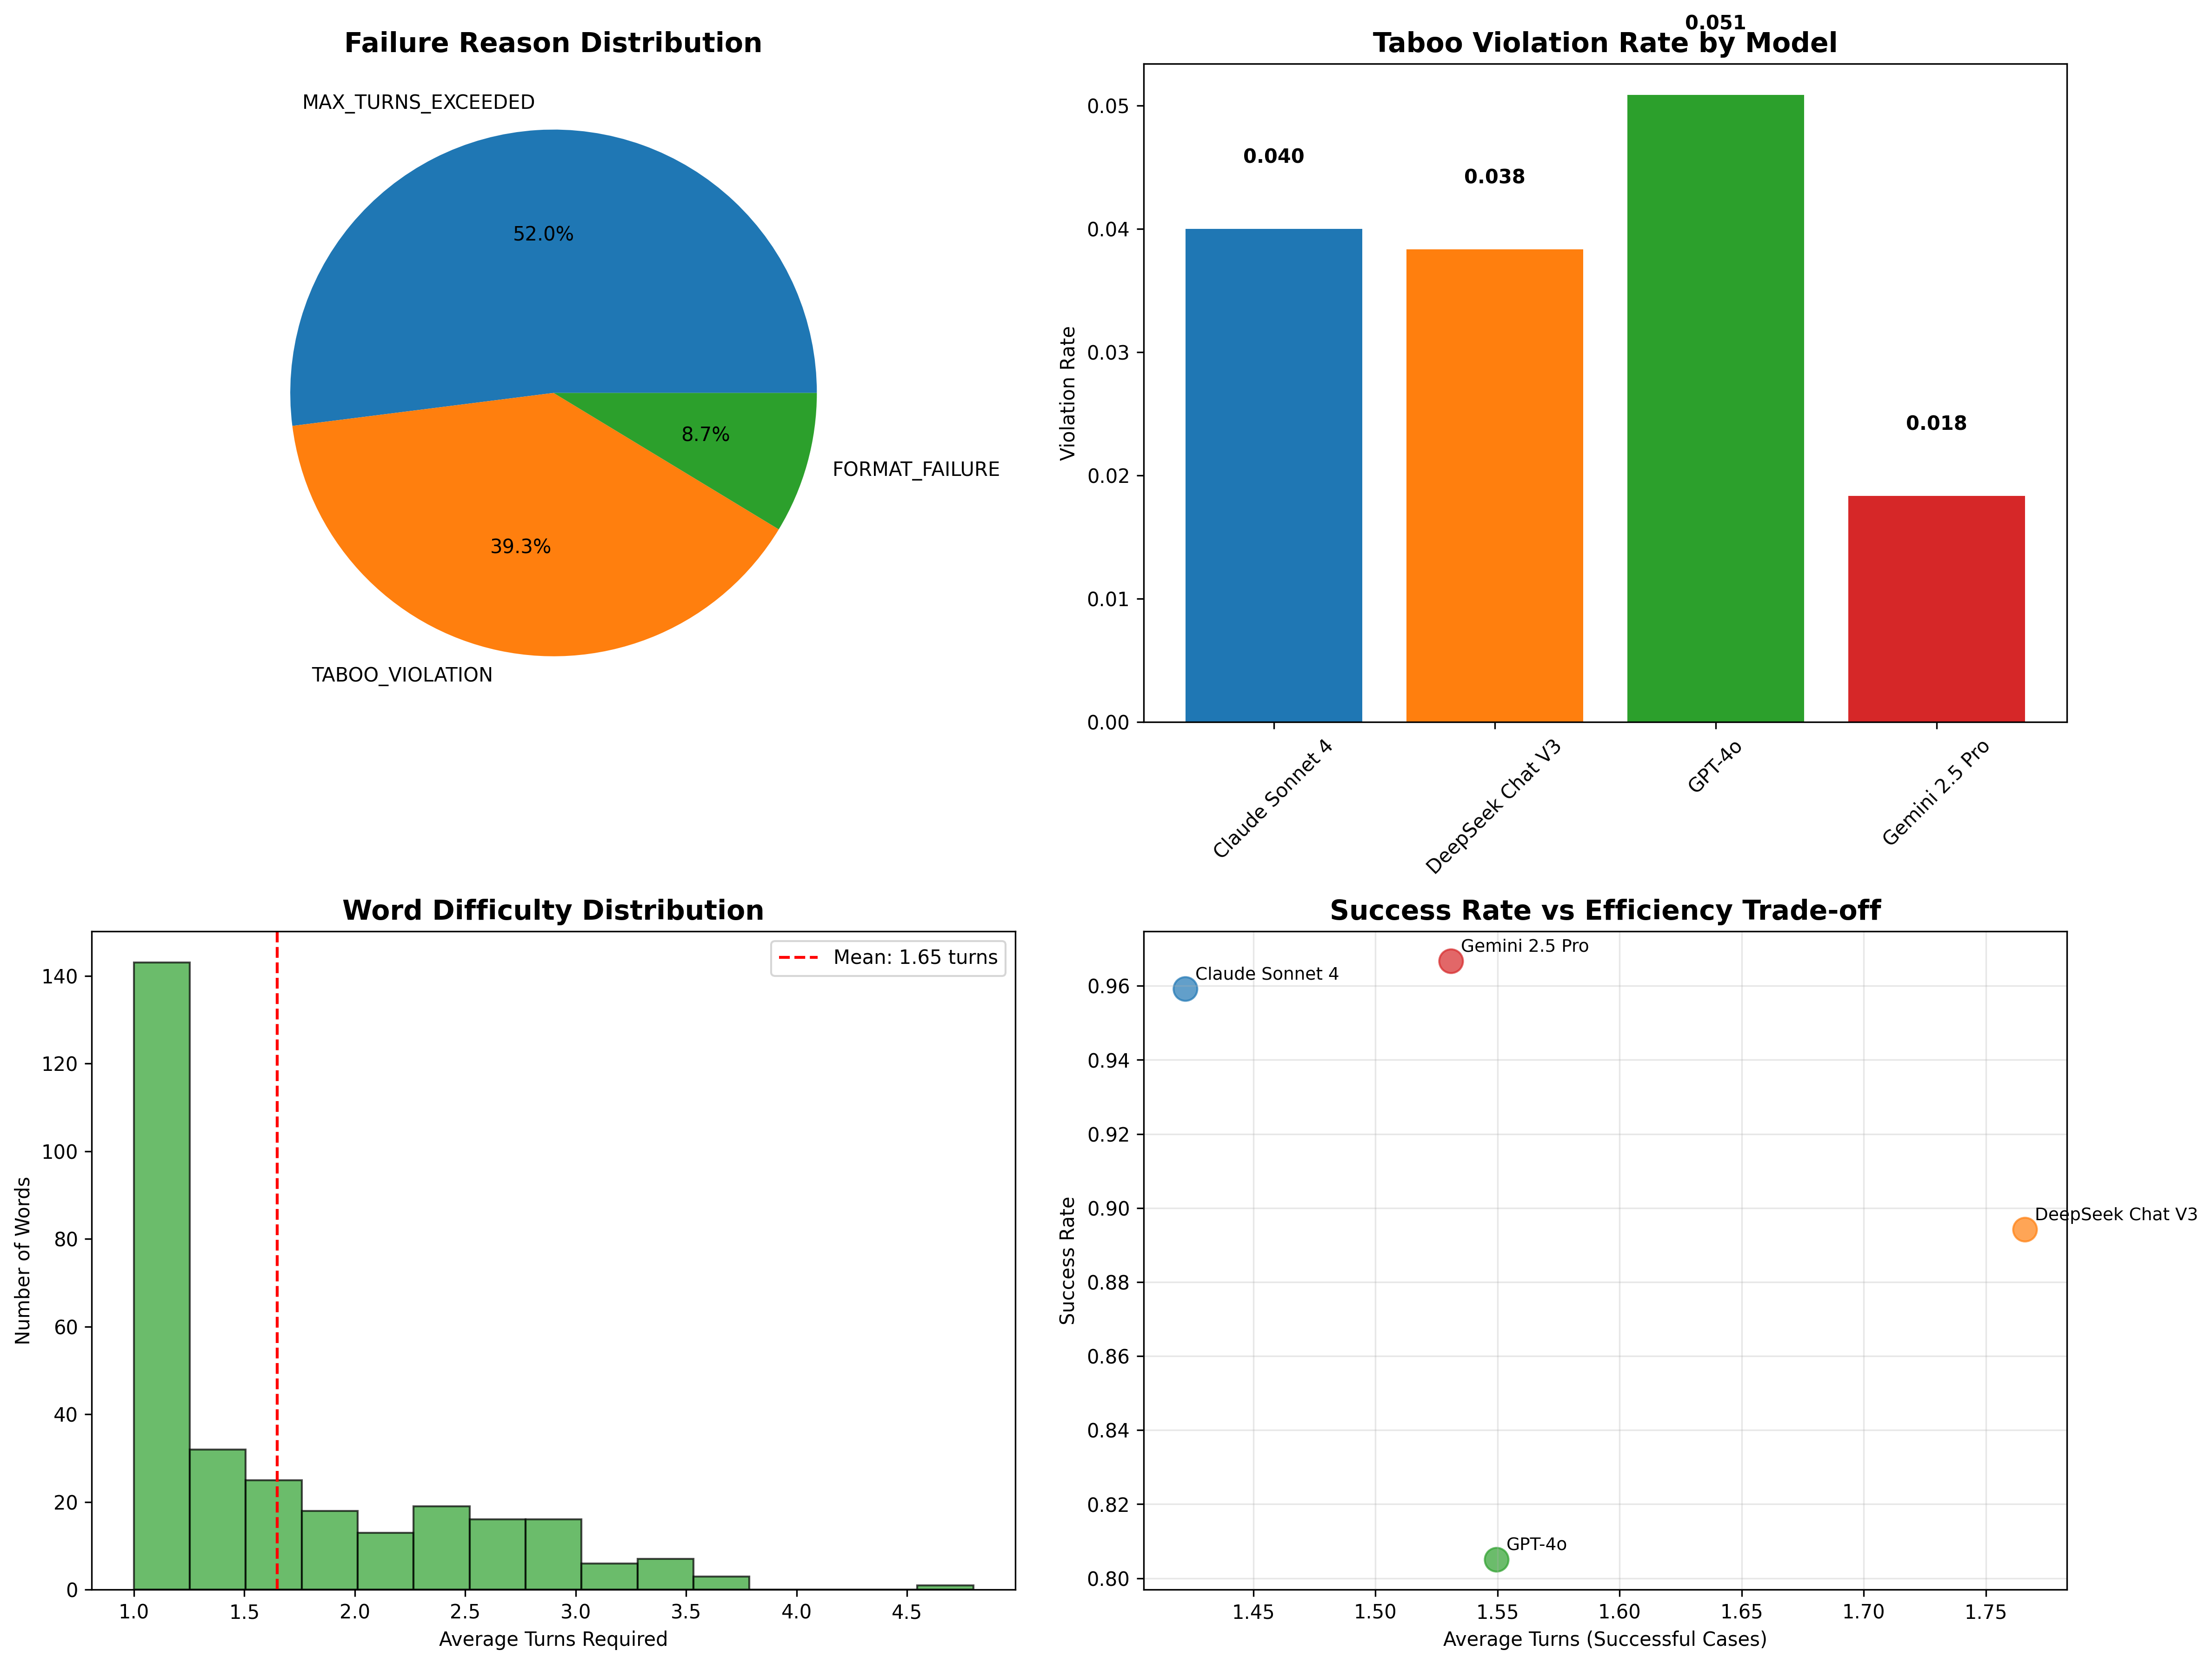
\includegraphics[width=\textwidth]{comprehensive_figures/figure6_error_analysis.png}
\caption{Error Analysis}
\end{figure}
\end{column}
\end{columns}
\end{frame}

%==============================================
% 4. Key Findings
%==============================================
\section{Key Findings}

\begin{frame}{Key Findings: Theoretical Implications}
\begin{columns}[c]
\begin{column}{0.5\textwidth}
\begin{alertblock}{Major Theoretical Contributions}
\begin{itemize}
    \item \textbf{Frequency Over Domain}: Word frequency is more predictive than domain knowledge
    \item \textbf{Constraint Adherence}: Models show systematic patterns in constraint violations
    \item \textbf{Creative Adaptation}: LLMs demonstrate varying degrees of linguistic creativity
\end{itemize}
\end{alertblock}

\begin{block}{Implications for Cognitive Science}
\begin{itemize}
    \item Models exhibit human-like frequency effects in language processing
    \item Constrained generation reveals limits of semantic representation
    \item Creative language use requires both constraint awareness and flexibility
\end{itemize}
\end{block}

\begin{block}{Implications for AI Development}
\begin{itemize}
    \item Training data frequency distribution critically affects performance
    \item Constraint-following capabilities vary significantly across models
    \item Need for specialized training on constrained communication tasks
\end{itemize}
\end{block}
\end{column}

\begin{column}{0.48\textwidth}
\begin{figure}
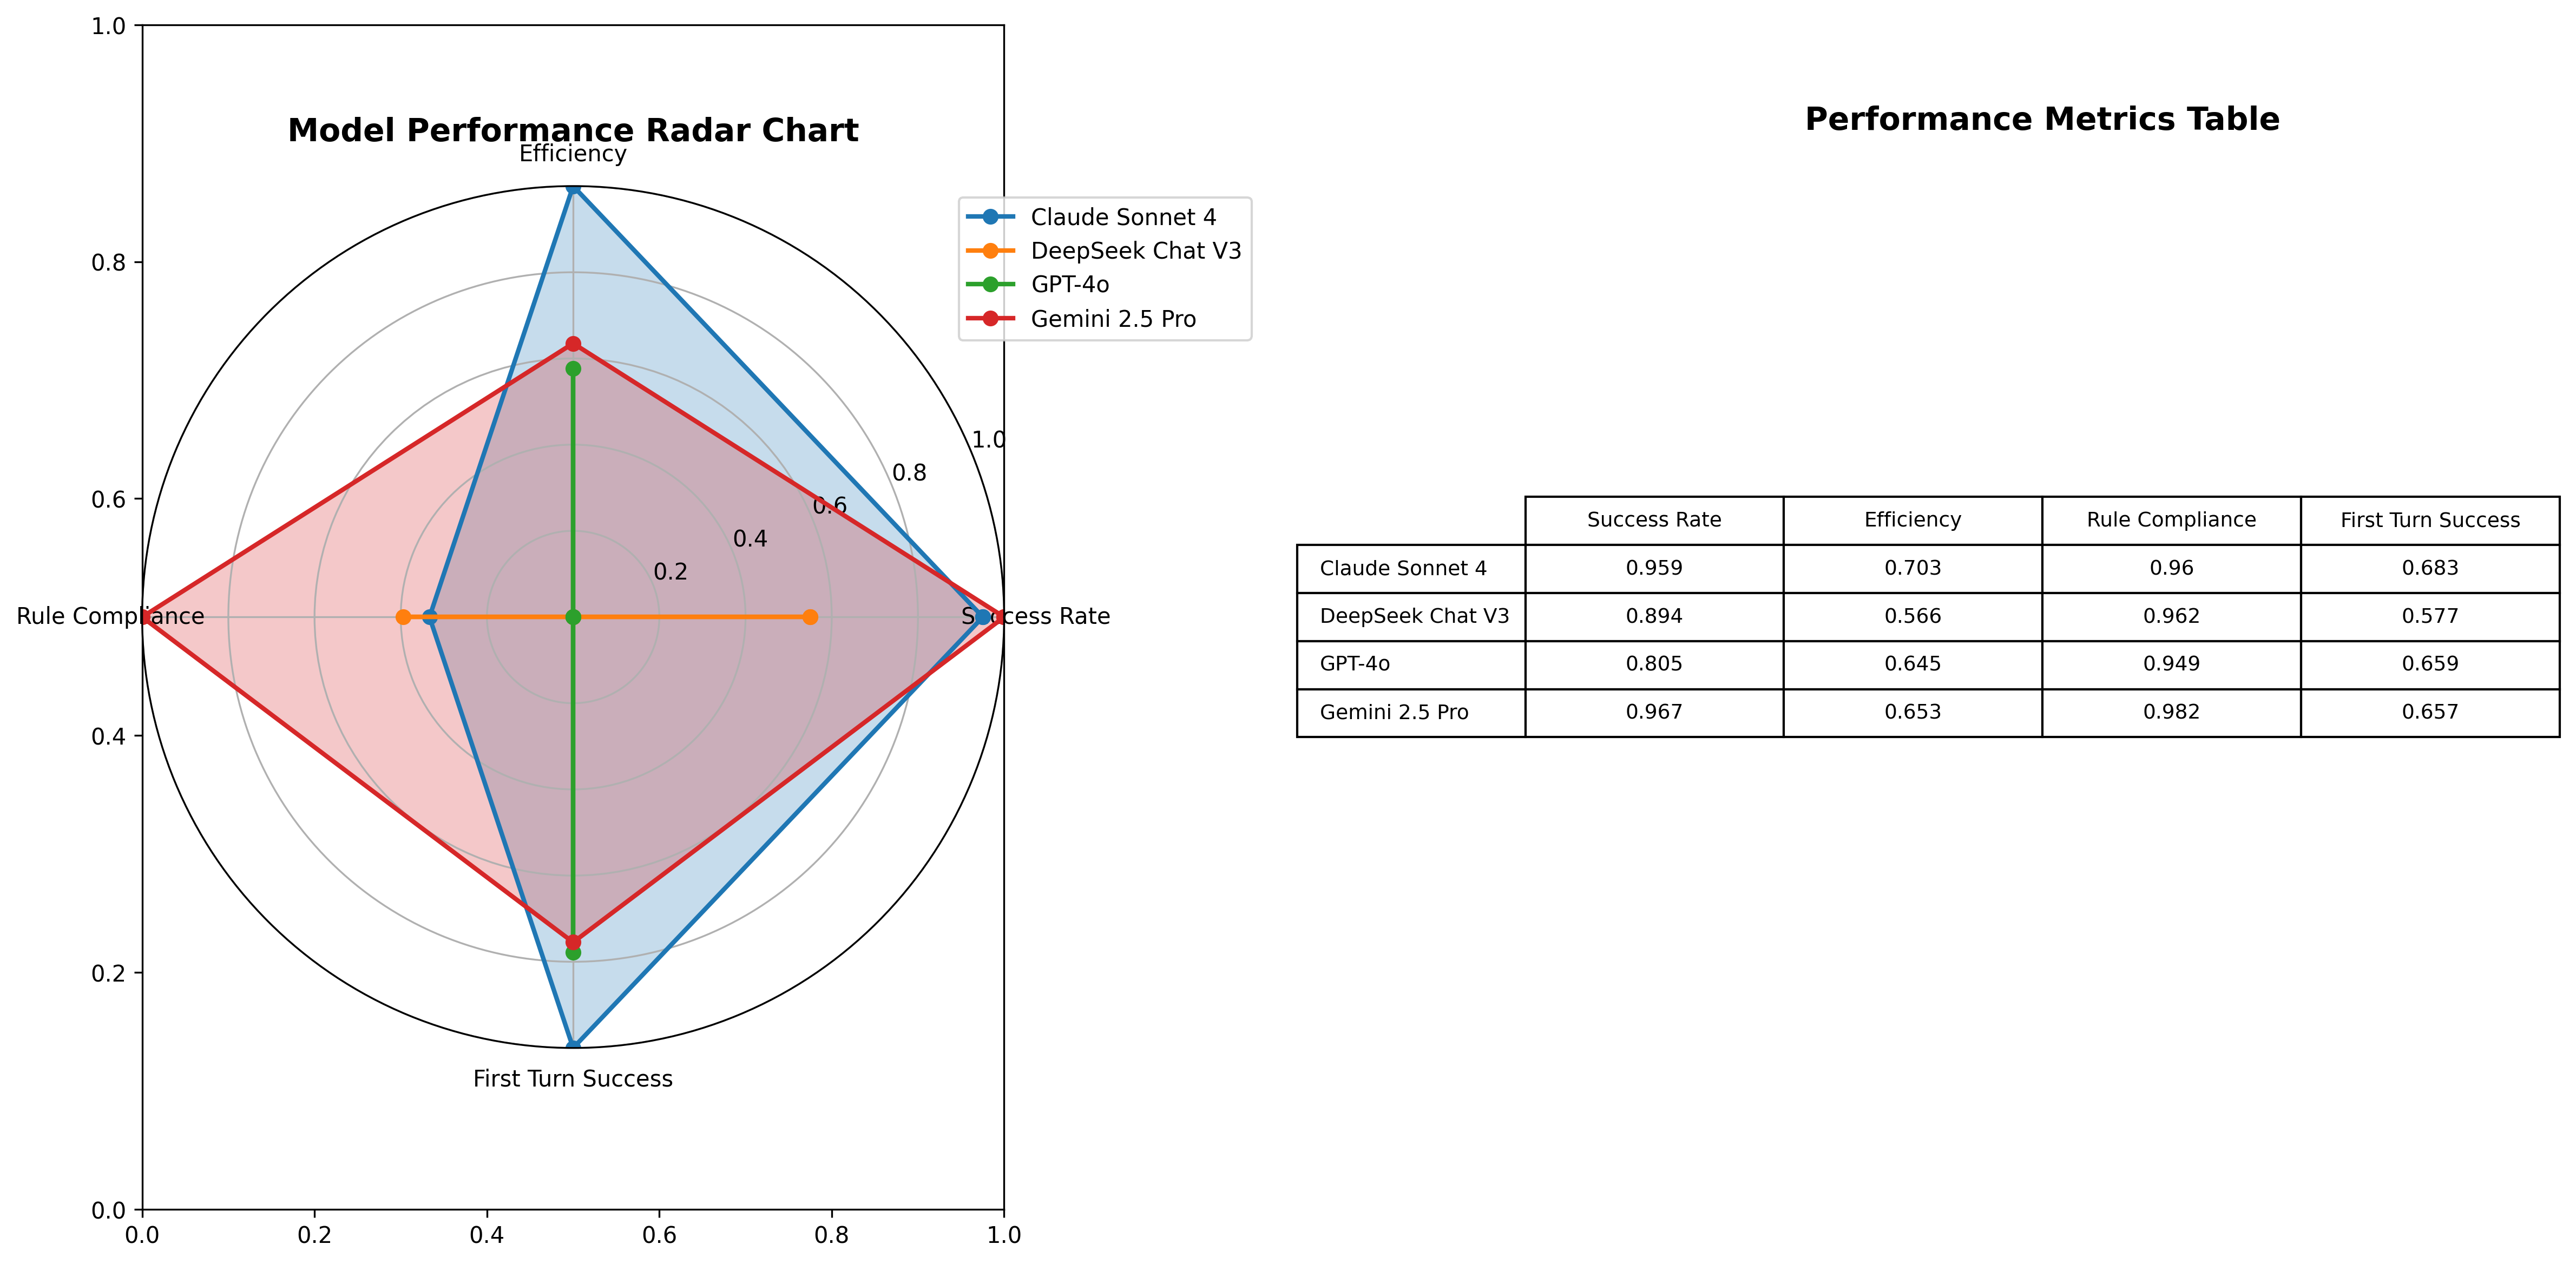
\includegraphics[width=\textwidth]{comprehensive_figures/figure7_radar.png}
\caption{Model Performance Radar Chart}
\end{figure}
\end{column}
\end{columns}
\end{frame}

\begin{frame}{Key Findings: Methodological Contributions}
\begin{block}{Novel Evaluation Framework}
\begin{itemize}
    \item First systematic Taboo game evaluation for LLMs
    \item Multi-dimensional analysis combining linguistic and performance metrics
    \item Reproducible methodology for comparative model assessment
\end{itemize}
\end{block}

\begin{block}{Empirical Insights}
\begin{itemize}
    \item Established performance hierarchy across 4 major LLMs
    \item Identified key linguistic factors affecting performance
    \item Revealed frequency-domain interaction effects
\end{itemize}
\end{block}

\begin{exampleblock}{Future Research Directions}
Framework can be extended to other constrained generation tasks and language models
\end{exampleblock}
\end{frame}

%==============================================
% 5. Discussion & Analysis
%==============================================
\section{Discussion \& Analysis}

\begin{frame}{Discussion \& Analysis: Theoretical Implications}
\begin{block}{Linguistic Processing Insights}
\begin{itemize}
    \item Models demonstrate frequency-based processing similar to humans
    \item Constraint adherence requires explicit instruction following
    \item Creative generation emerges from semantic flexibility
\end{itemize}
\end{block}

\begin{block}{Model Architecture Implications}
\begin{itemize}
    \item Transformer attention mechanisms affect constraint tracking
    \item Training data distribution impacts domain performance
    \item Model size correlates with constraint adherence quality
\end{itemize}
\end{block}

\begin{alertblock}{Broader AI Implications}
Understanding constraint-following capabilities is crucial for reliable AI deployment
\end{alertblock}
\end{frame}

%==============================================
% 6. Limitations & Future Work
%==============================================
\section{Limitations \& Future Work}

\begin{frame}{Limitations \& Future Work: Current Limitations}
\begin{block}{Methodological Limitations}
\begin{itemize}
    \item Limited to English language evaluation
    \item Focus on single-turn constraint following
    \item Subjective elements in human evaluation
    \item Limited domain coverage (5 domains)
\end{itemize}
\end{block}

\begin{block}{Technical Limitations}
\begin{itemize}
    \item Evaluation limited to 4 models
    \item No fine-tuning experiments conducted
    \item Limited analysis of failure mode patterns
    \item Constraint complexity not systematically varied
\end{itemize}
\end{block}

\begin{block}{Scope Limitations}
\begin{itemize}
    \item Single game type (Taboo) evaluated
    \item No comparison with human performance
    \item Limited exploration of prompt engineering effects
\end{itemize}
\end{block}
\end{frame}

\begin{frame}{Limitations \& Future Work: Future Research Directions}
\begin{block}{Immediate Extensions}
\begin{itemize}
    \item Expand to multilingual evaluation
    \item Include more recent LLMs in comparison
    \item Develop automated evaluation metrics
    \item Systematic prompt engineering studies
\end{itemize}
\end{block}

\begin{block}{Long-term Research Goals}
\begin{itemize}
    \item Develop specialized training methods for constraint adherence
    \item Create comprehensive benchmark suite for constrained generation
    \item Investigate neural mechanisms underlying constraint following
    \item Explore applications in interactive AI systems
\end{itemize}
\end{block}

\begin{exampleblock}{Broader Impact}
Results inform development of more reliable and controllable AI communication systems
\end{exampleblock}
\end{frame}

%==============================================
% 7. Conclusion
%==============================================
\section{Conclusion}

\begin{frame}{Conclusion: Summary of Contributions}
\begin{block}{Key Empirical Findings}
\begin{itemize}
    \item Established clear performance hierarchy: Gemini 2.5 Pro > Claude Sonnet 4 > DeepSeek Chat V3 > GPT-4o
    \item Demonstrated that 65.9\% of apparent domain effects are word frequency effects
    \item Identified linguistic factors affecting constrained generation performance
\end{itemize}
\end{block}

\begin{block}{Methodological Innovations}
\begin{itemize}
    \item First comprehensive LLM evaluation using Taboo games
    \item Novel multi-dimensional analysis framework
    \item Reproducible evaluation methodology for constraint-following tasks
\end{itemize}
\end{block}

\begin{block}{Theoretical Contributions}
\begin{itemize}
    \item Revealed frequency-domain interaction effects in LLM performance
    \item Demonstrated systematic patterns in constraint violation behaviors
    \item Provided insights into creative language generation under constraints
\end{itemize}
\end{block}
\end{frame}

\begin{frame}{Conclusion: Key Takeaways}
\begin{alertblock}{For AI Researchers}
\begin{itemize}
    \item Word frequency is more predictive than domain knowledge
    \item Constraint adherence varies significantly across models
    \item Multi-dimensional evaluation reveals nuanced performance patterns
\end{itemize}
\end{alertblock}

\begin{alertblock}{For Practitioners}
\begin{itemize}
    \item Choose models based on constraint-following requirements
    \item Consider frequency effects when designing evaluation datasets
    \item Implement systematic evaluation for constrained generation tasks
\end{itemize}
\end{alertblock}

\begin{exampleblock}{Future Impact}
This work establishes foundation for more reliable and controllable AI systems
\end{exampleblock}
\end{frame}

\begin{frame}[plain]
\begin{center}
\huge Thank You!

\vspace{1cm}

\Large Questions \& Discussion

\vspace{1cm}

\normalsize
\textbf{Contact:} your.email@university.edu\\
\textbf{Repository:} github.com/username/taboo-llm-eval
\end{center}
\end{frame}

\end{document} 